\section{Inleiding}

\subsection{Opbouw van de Cursus}

De cursus is onderverdeeld in een deel over micro-economie, en een deel over macro-economie.

\begin{leftbar}
\par\entrystyled{micro-economie}{Micro-economie} (H1-13) gaat eerder over het standpunt van het individu ; \textit{`hoe maximaliseer ik mijn winst', `hoe beheer ik best mijn budget'}, ... ? Men spreekt van \term{elementaire veranderlijken}, veranderlijken die men onmiddellijk, zonder berekening kan waarnemen (eg. prijzen, inkomens, ...). Geld is hier niet nodig, men heeft het over relatieve prijzen. \\
Het micro-economisch perspectief is optimistisch, het gaat over het bereiken van een evenwicht, zonder overheidsinterventie. De overheid heeft een bijrol. \\
\par\entrystyled{macro-economie}{Macro-economie} (H15-26) gaat over een helicopter-perspectief ; men spreekt over het land, de wereld, ... Hier spreekt men eerder over aggregaten (zoals het bruto nationaal product, de export, ...) en gemiddelden (zoals de prijsindexering). Geld is nu wel belangrijk, omdat men het onder andere heeft over prijsniveau's. \\
Bij macro-economie komen onevenwichten aan bod. De overheid speelt dan ook een hoofdrol.\\
\end{leftbar}

\par\noindent Naast dit onderscheid heeft men het ook over een ander onderscheid : statica versus dynamica ...

\begin{leftbar}
\par Bij een \term{statisch perspectief} (H13, 24-26) gaat men ervan uit dat de productiefactoren (arbeid en kapitaal) gegeven zijn, en vraagt men zich af hoe men deze optimaal aanwendt (eg. \textit{`hoe minimaliseert men werkloosheid?'}).\\
Men gaat ervan uit dat de economische agenten rationeel (optimaliserend) zijn, en dat ze vrijwillig ruilen. Een vrije marktwerking dus. Toch is er - in tweede orde - nood aan overheidsinterventie, zoals bij publieke goederen en externe effecten, of bij herverdeling. Een wereldregering is er niet.\\
\par Bij een \term{dynamisch perspectief} (H17-18, 23) heeft men het over de systematische toename van de productiemiddelen (bedrijven worden groter door investeringen etc.). Er is een toename van het bruto-binnenlands product, men heeft het over economische groei. Korte-termijn veranderingen van deze groei noemt men conjunctuurschommelingen.
\end{leftbar}

\par\noindent Een laatste onderscheid is dat tussen de re\"ele en de financi\"ele sector :

\begin{leftbar}
\par De \entrystyled{reele sector}{re\"ele sector} vormt de kern en omvat dus productie van goederen en diensten, de productie-eenheden (bedrijven, overheden, VZW's, gezinnen), ... \\
\par De \entrystyled{financiele sector}{financi\"ele sector} omgeeft die kern. Hier wordt een algemeen aanvaard ruilmiddel, het geld, gecre\"eerd, en wordt lenen en ontlenen mogelijk gemaakt. De centrale bank en de commerci\"ele banken spelen hier de hoofdrol.\\
Merk op dat geld niet de essentie van de economie is. Welvaart is dat wel.\\
Het is in de financi\"ele sector dat financi\"ele crisissen kunnen ontstaan omdat schuldenaars hun schulden niet kunnen terugbetalen, waarna hun schuldeisers dat ook niet meer kunnen, enzovoort (de bankencrisis in de VS in 2007 is een voorbeeld).
\end{leftbar}

\subsection{Optimaliserende Economische Agenten}\label{sec:h0oea}

Doorheen de cursus gaat men uit van rationele, goed ge\"informeerde economische agenten die handelen uit eigenbelang. Men spreekt van `optimaliserend gedrag', en men noemt zo'n agent een \entry{homo economicus} (`\entry{econ}').\\
De econ kiest de beste oplossing (dit gaat meestal over een hoeveelheid). Hij koopt, verkoopt, rekruteert, werkt, ontleent en leent tot de laatste eenheid hem evenveel opbrengt als hij hem kost. Met andere woorden, tot zijn \entry{marginale opbrengst}\footnote{Voor de consument is deze gelijk aan zijn \term{marginale betalingsbereidheid} $MBB$.} gelijk wordt aan zijn \entry{marginale kost} : $MO=MK$. \\

\par\noindent Het woord `\textit{marginaal}' verwijst naar de laatste eenheid. De marginale kost is dus de kost van nog \'e\'en bijkomende eenheid, of de \textit{stijging} van de grafiek van de totale kost $TK$ bij oplopende hoeveelheid $q$. \\

\par In figuur \ref{fig:plot1} wordt de marginale betalingsbereidheid van een consument aan de linkerkant afgebeeld, en rechts diezelfde betalingsbereidheid naast de marginale kost (de werkelijke prijs $P$, hier constant). Om een evenwicht te bereiken zal de econ dus producten blijven kopen tot $MO=MBB=P=MK$ (in $q=5$).

\begin{figure}
\centering
\captionsetup{justification=centering,margin=2cm}
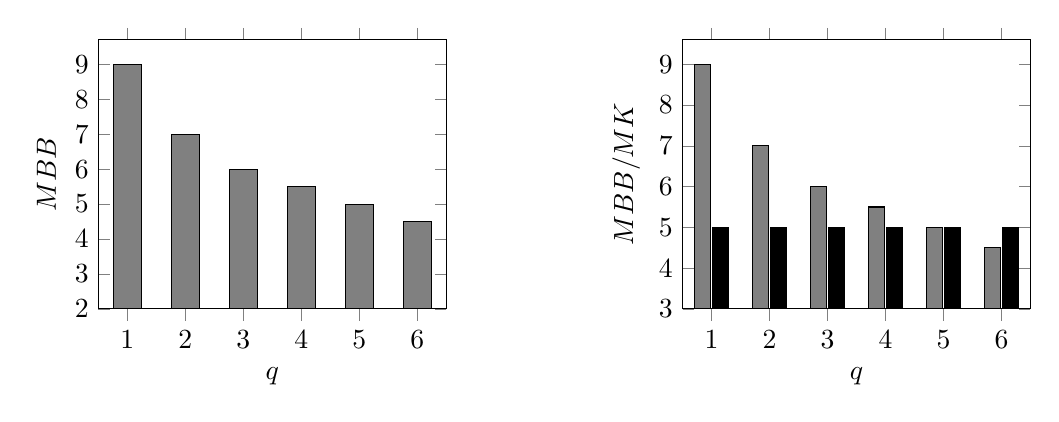
\begin{tikzpicture}
	\begin{axis}[name=left,xlabel=$q$, ylabel=$MBB$, ymin=2,xtick={1,...,7}, ytick={0,...,9}, width=6cm, height=5cm,ybar=2*\pgflinewidth]
		\addplot[ybar,fill=gray] coordinates {(1,9)(2,7)(3,6)(4,5.5)(5,5)(6,4.5)};
	\end{axis}
	\begin{axis}[at={(left.north east)},anchor=north west,xshift=3cm,xlabel=$q$, ylabel=$MBB/MK$, ymin=3,xtick={1,...,6}, ytick={0,...,10}, width=6cm, height=5cm,bar width=0.2cm,ybar=2*\pgflinewidth]
		\addplot[ybar,fill=gray] coordinates {(1,9)(2,7)(3,6)(4,5.5)(5,5)(6,4.5)};
		\addplot[ybar,fill=black] coordinates {(1,5)(2,5)(3,5)(4,5)(5,5)(6,5)};
	\end{axis}
\end{tikzpicture}
\caption{(a) De marginale betalingsbereidheid van de consument, \\(b) Diezelfde betalingsbereidheid naast de feitelijke (constante) prijs}
\label{fig:plot1}
\end{figure}

\par Nu illustreert figuur \ref{fig:plot1} wel een discrete variatie ; men koopt per eenheid. Per fles wijn, bijvoorbeeld. Bij continue variatie kan men ook andere hoeveelheden aankopen, zoals een milliliter wijn of minder. De grafiek wordt dan een curve. En dan is de marginale betalingsbereidheid de \entry{afgeleide} $\frac{dTBB}{dq}$ met $TBB$ de totale betalingsbereidheid\footnote{Meer hierover in de appendix.}.

\begin{figure}
\vspace{0.5cm}
\centering
\captionsetup{justification=centering,margin=2cm}
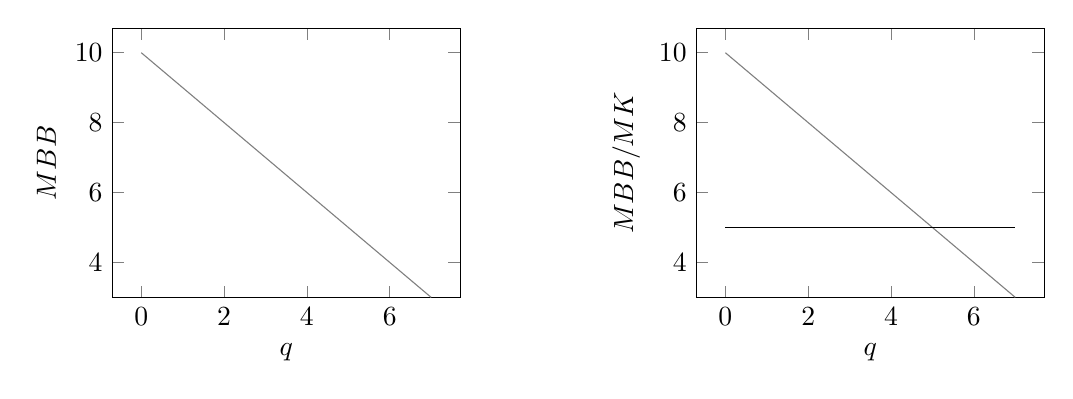
\begin{tikzpicture}
	\begin{axis}[name=left,xlabel=$q$, ylabel=$MBB$, ymin=3,width=6cm, height=5cm]
		\addplot[gray, samples=100, domain=0:7] {10-x};
	\end{axis}
	\begin{axis}[at={(left.north east)},anchor=north west,xshift=3cm,xlabel=$q$, ylabel=$MBB/MK$, ymin=3,width=6cm, height=5cm,bar width=0.2cm]
		\addplot[gray, samples=100, domain=0:7] {10-x};
		\addplot[black, samples=100, domain=0:7] {5};
	\end{axis}
\end{tikzpicture}
\caption{Hetzelfde als figuur \ref{fig:plot1}, maar bij continue variatie}
\label{fig:plot2}
\end{figure}

\subsection{Humans versus Econs}

In de werkelijkheid zijn er geen econs, maar mensen van vlees en bloed. Er wordt dus niet werkelijk geoptimaliseerd door individu's en overheden (er is `\textit{bounded rationality}', en `\textit{bounded will power}'). Het zijn de psychologen, politicologen en geschiedkundigen die dan bijkomend inzicht kunnen leveren.\\

\par In deze context spreekt men ook van \entry{intrinsieke motivatie} en \entry{extrensieke motivatie}. Het eerste ontstaat vanuit de persoon zelf, het tweede ontstaat door een externe bron (zoals het vooruitzicht op een beloning) ; het eerste gaat om het spel, het tweede om de knikkers.